 \begin{center}\begin{large} Homework Problems 2 (Matrices) \end{large}\end{center}
 \bigskip




\begin{problem}
Match the descriptions a)-f) with matrices 1)-6):
\smallskip 
\textit{Descriptions:} 

\begin{enumerate}
    \item[a) ] Rotation by $70^\circ$
    \item[b) ] Not changing anything
    \item[c) ] Flipping around the $x$-axis
    \item[d) ] Stretching out $5$ times in $y$-direction
    \item[e) ] Sending all vectors onto the line $y=6x$
    \item[f) ] Sending all vectors onto the line $y=6x+1$
\end{enumerate}

\textit{Matrices:} 

\begin{enumerate}
    \item[1) ] $\begin{bmatrix}
        1&0\\0&5
    \end{bmatrix}$
    \item[2) ] Such matrix does not exist
    \item[3) ] $\begin{bmatrix}
        1&0\\0&1
    \end{bmatrix}$
    \item[4) ] $\begin{bmatrix}
        0.342 & -0.939\\
         0.939& 0.342
    \end{bmatrix}$
    \item[5) ] $\begin{bmatrix}
        1&0\\0&-1
    \end{bmatrix}$
    \item[6) ] $\begin{bmatrix}
        3&-1\\18&-6
    \end{bmatrix}$
\end{enumerate}

{\small \textit{Hint: Compute the determinants.}
    }
\end{problem}

\medskip 

\begin{problem}
    What is the determinant of the matrix
    
    \begin{enumerate}
    \item[a) ] which rotates everything by $14^\circ$ and stretches $1.5$ times in the $x$-direction,

 \item[b) ] which does the inverse of a),

 \item[c) ] which sends $[1 \,\,\,\,0]$ to $[2 \,\,\,\,4]$ and $[0\,\,\,\,1]$ to $[-1\,\,\,0]$,

 \item[d) ] which has the form $\begin{bmatrix}
     2 & 3 \\ 2 &1
 \end{bmatrix}$,
 
        \item[e) ] which has the form  $=\begin{bmatrix}
        8&3&5\\1&4&2\\-4&0&4   \end{bmatrix}$,

        \item[f) ] which is the matrix of e) raised to the power $3$.
    \end{enumerate}
\end{problem}
\medskip


\begin{problem}
Fill in the missing entries of 
\[
\begin{bmatrix}
    2 & * \\ -1 & *
\end{bmatrix}
\]
if it
    \begin{enumerate}
        \item[a) ] stretches $[0 \,\,\,\,1]$ by $2$ times,
        
        \item[b) ] has trace $2$ and determinant $3$,
        
        \item[c) ] has eigenvalues $1$ and $5$.
    \end{enumerate}

\end{problem}
\medskip

\begin{problem}%[\textbf{optional, not graded}]
    A subspace of which dimension (at most) can you construct with the vectors:
    \begin{enumerate}
        \item[a) ] $\vv_1=\begin{bmatrix}6\\1\\5\end{bmatrix},  \vv_2=\begin{bmatrix}
            2\\3\\2
        \end{bmatrix}$,

        
        \item[b) ] $\vv_1=\begin{bmatrix}6\\2\end{bmatrix},  \vv_2=\begin{bmatrix}
            1\\3
        \end{bmatrix},  \vv_3=\begin{bmatrix}
            5\\2
        \end{bmatrix}$,
        
        \item[c) ] $\vv_1=\begin{bmatrix}4\\1\\2\end{bmatrix},  \vv_2=\begin{bmatrix}
            -4\\2\\-1
        \end{bmatrix},  \vv_3=\begin{bmatrix}
            8\\-1\\7
        \end{bmatrix}$,
        
        \item[d) ] $\vv_1=\begin{bmatrix}3\\-2\\1\end{bmatrix},  \vv_2=\begin{bmatrix}
            6\\-4\\4
        \end{bmatrix}$.
        
    \end{enumerate}
\end{problem}

\medskip 

\begin{problem}
    Find the eigenvalues and eigenvectors of the following matrices:

    \begin{enumerate}
        \item[a) ] $A=\begin{bmatrix}
            1&2\\0&1\end{bmatrix}$,

        \item[b) ] $B=\begin{bmatrix}
            2&1\\1&2
        \end{bmatrix}$,
        
        \item[c) ] $C=\begin{bmatrix}
            8 & 1 \\ 8 & 1
        \end{bmatrix}$,
        
        \item[d) ] $D=\begin{bmatrix}
-1&0&0\\0&1&0\\0&0&3        \end{bmatrix}$.
    \end{enumerate}

    You may use any of the techniques (characteristic polynomial / trace and determinant / columns-basis relationship) but try to also think of the problem visually.
\end{problem}


\medskip 

\begin{problem}
    If you take the unit circle $x^2+y^2=1$ (i.e. the circle with center at $(0,0)$ and radius $1$) and stretch it out $2$ times along the $x$-axis, you will get an \textit{ellipse}. What is its area equal to?

    \begin{figure}[h]
        \centering
        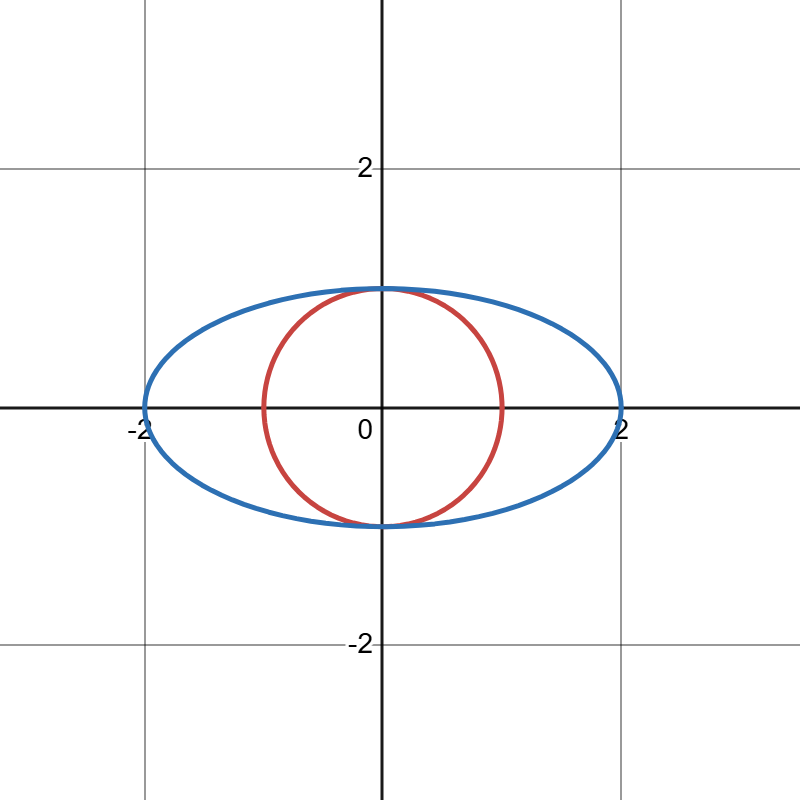
\includegraphics[width=0.5\linewidth]{ellipse.png}
    \end{figure}

    (Additional:) Can you generalize the result to derive a formula for the area of ellipse?
\end{problem}


\medskip 

\begin{problem}
    It is known that the matrix 
    \[
    A=\begin{bmatrix}
        4 & -8 \\ 1 & 2
    \end{bmatrix}
    \]
    sends a certain vector $\mathbf{v}$ to
\begin{enumerate}
    \item[a) ] $\begin{bmatrix}
        1 \\2
    \end{bmatrix}$,
    \item[b) ] $\begin{bmatrix}
        3 \\ 4
    \end{bmatrix}$.
\end{enumerate}
Can you find the vector $\mathbf{v}$?


\end{problem}



\medskip 

\begin{problem}[\textbf{additional}]
    Consider the $5 \times 5$ matrix 
    \[
    A=\begin{bmatrix}
        a_1 & 0 & 0 & 0 & 0 \\
        0 & a_2 & 0 & 0 & 0 \\
        0 & 0 & a_3 & 0 & 0 \\
        0 & 0 & 0 & a_4 & 0 \\
        0 & 0 & 0 & 0 & a_5 
    \end{bmatrix}
    \]
    where $a_1, \dots, a_5$ are some fixed positive numbers. 
    \begin{enumerate}
        \item[a) ] What is the standard basis of $\mathbb{R}^5$?
        
        \item[b) ] Where does $A$ send the standard basis vectors of $\mathbb{R}^5$?

        \item[c) ] What do you think is the determinant of $A$?
        
        \item[d) ] What do you think are the eigenvalues and eigenvectors of $A$?
    \end{enumerate}


\end{problem}





        
        